% !TeX root = Report.tex
\documentclass[a4paper,12pt]{report}
% !TeX root = main.tex
%_______________________________ Packages ______________________________
\usepackage[utf8]{inputenc}
\usepackage[french]{babel}       %for language
\usepackage{float} %for H
\usepackage{blindtext}                                                  %for Dummy Text
\usepackage[a4paper,top=2.5cm,bottom=2.5cm,left=2.75cm,right=2.75cm]{geometry}    %for document shape
\usepackage{graphicx}                                                   %images
\usepackage{enumitem}                                                   % Used to compact lists
\usepackage{fancyhdr}                                                   %fancy headers
\usepackage{amsmath}                                                    %maths
\usepackage{titling}                                                    %for a pretitle f maketitle
\usepackage{tikz}
\usepackage{fancybox}
\usepackage{tabularx}
\usepackage{wrapfig}
\usepackage{titlesec}
\usepackage{hyperref}
\usepackage{indentfirst}
\usepackage[footnote]{acronym}

%_______________________________________________________________________
%_______________________________ for font ______________________________
%\renewcommand{\familydefault}{\sfdefault}     
\selectlanguage{french}
%_______________________________________________________________________
%___________________________ for fancy pages ___________________________
\pagestyle{fancy}   
\renewcommand{\headrulewidth}{1pt}
\renewcommand{\footrulewidth}{1pt}
\fancyhead[R,L]{\chaptername \  \thechapter}
\fancyhead[LE,RO]{\rightmark} 
\addto\captionsenglish{% Replace "english" with the language you use
  \renewcommand{\contentsname}%
    {Table des matières}%
}


 %%%%********************************************************************
\definecolor{quotemark}{gray}{0.7}
\makeatletter
\def\fquote{%
    \@ifnextchar[{\fquote@i}{\fquote@i[]}%]
           }%
\def\fquote@i[#1]{%
    \def\tempa{#1}%
    \@ifnextchar[{\fquote@ii}{\fquote@ii[]}%]
                 }%
\def\fquote@ii[#1]{%
    \def\tempb{#1}%
    \@ifnextchar[{\fquote@iii}{\fquote@iii[]}%]
                      }%
\def\fquote@iii[#1]{%
    \def\tempc{#1}%
    \vspace{1em}%
    \noindent%
    \begin{list}{}{%
         \vspace{3.6cm}
         \setlength{\leftmargin}{0.1\textwidth}%
         \setlength{\rightmargin}{0.1\textwidth}%
                  }%
         \item[]%
         \begin{picture}(0,0)%
         \put(-15,-5){\makebox(0,0){\scalebox{3}{\textcolor{quotemark}{``}}}}%
         \end{picture}%
         \begingroup\itshape}%
 %%%%********************************************************************
 \def\endfquote{%
 \endgroup\par%
 \makebox[0pt][l]{%
 \hspace{0.8\textwidth}%
 \begin{picture}(0,0)(0,0)%
 \put(15,15){\makebox(0,0){%
 \scalebox{3}{\color{quotemark}''}}}%
 \end{picture}}%
 \ifx\tempa\empty%
 \else%
    \ifx\tempc\empty%
       \hfill\rule{100pt}{0.5pt}\\\mbox{}\hfill\tempa,\ \emph{\tempb}%
   \else%
       \hfill\rule{100pt}{0.5pt}\\\mbox{}\hfill\tempa,\ \emph{\tempb},\ \tempc%
   \fi\fi\par%
   \vspace{0.5em}%
 \end{list}%
 }%
 \makeatother
 %%%%********************************************************************


\bibliographystyle{plain}

\newenvironment{remerciements}
{%begin
    \begin{titlepage}
    \hspace{0pt}
    \vfill
    \begin{center}
        \textbf{\Large Remerciement}
    \end{center}
    \hrule\bigskip
}
{%end
    \begin{center}
        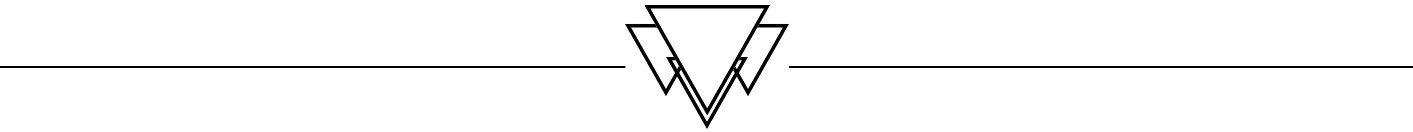
\includegraphics[width = \linewidth]{images/zwa9a line.png}
    \end{center}
    \vfill
    \hspace{0pt}
    \end{titlepage}
}


\newenvironment{resume}
{%begin
    
    \begin{titlepage}
    \hspace{0pt}
    \vfill
    \begin{center}
        \textbf{\Large Résumé}
    \end{center}
    \hrule\bigskip
}
{%end
    \begin{center}
        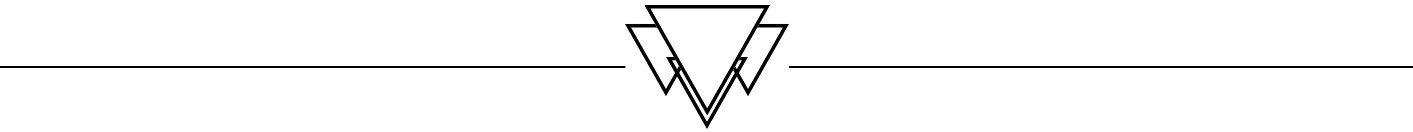
\includegraphics[width = \linewidth]{images/zwa9a line.png}
    \end{center}
    \vfill
    \hspace{0pt}
    \end{titlepage}
}

\newenvironment{englishabstract}
{%begin
    \begin{titlepage}
    \hspace{0pt}
    \vfill
    \begin{center}
        \textbf{\Large Abstract}
    \end{center}
    \hrule\bigskip
}
{%end
    \begin{center}
        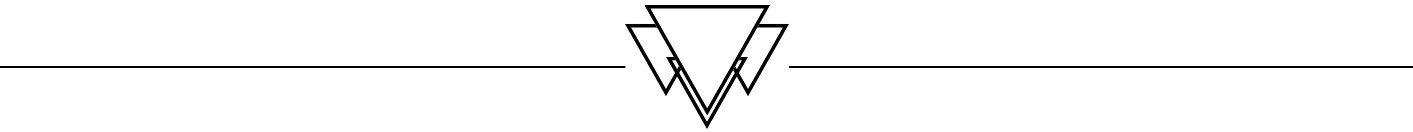
\includegraphics[width = \linewidth]{images/zwa9a line.png}
    \end{center}
    \vfill
    \hspace{0pt}
    \end{titlepage}
}



\newenvironment{introductiongenerale}
{%begin
    
    \begin{titlepage}
    \vspace*{1cm}
    \begin{center}
        \textbf{\Large Introduction Générale}
    \end{center}
    \hrule\bigskip
}
{%end
    \vfill
    \begin{center}
        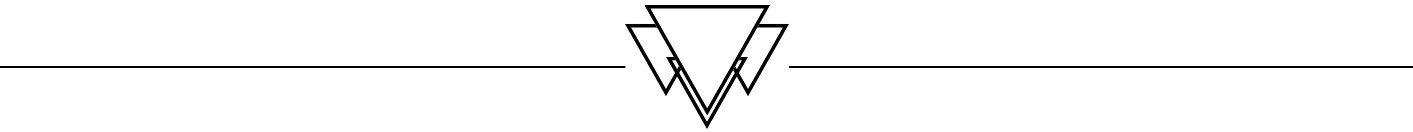
\includegraphics[width = \linewidth]{images/zwa9a line.png}
    \end{center}
    \vspace{3cm}
    \end{titlepage}
}

\newenvironment{conclusiongeneral}
{%begin
    
    \begin{titlepage}
    \vspace*{.5cm}
    \begin{center}
        \textbf{\Large Conclusion Finale}
    \end{center}
    \hrule\bigskip
}
{%end
    \vfill
    \begin{center}
        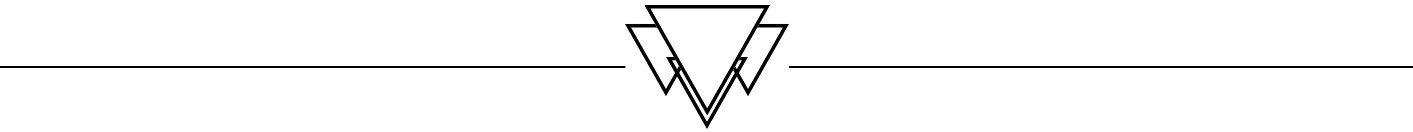
\includegraphics[width = \linewidth]{images/zwa9a line.png}
    \end{center}
    \vspace{3cm}
    \end{titlepage}
}


\begin{document}
    %================================COVER PAGE==============================
    \thispagestyle{empty} 
    \begin{titlepage}\label{TitlePäge}
\begin{center}
    \begin{figure}[!htb]
        \begin{minipage}{0.5\linewidth}
            
\includegraphics[width=0.58\linewidth]{logos/Um5-ENSIAS.png}
        \end{minipage}
        \hspace{1.8cm}
        \begin{minipage}{0.5\linewidth}
            
\includegraphics[width=0.84\linewidth]{logos/BCP.png}
        \end{minipage}
    \end{figure}
     
   \vspace*{1.6cm}

  \textsc{\huge \bfseries Projet de Fin d'Études}\\[1.3cm]
  \textsc{\small Filière}\\[1cm]
  \textsc{\huge \bfseries Génie Logiciel }\\[1.4cm]
  \textsc{\small Sujet}\\
  \begin{center}
 \rule{0.5\linewidth}{1pt}
 \end{center}
  \textsc{\huge \bfseries Automatisation du Registre du \\\vspace*{0.5cm} Traitement}
  \begin{center}
 \rule{0.5\linewidth}{1pt}
 \end{center}
 
 \vspace{2.8cm}
  
  \begin{minipage}{0.5\textwidth}
    \vspace{-6mm}
  \begin{flushleft} \large
    \emph{\bfseries Réalisé par}\\[0.3cm]
    Mehdi CHARIFE \\[0.5cm]
    \emph{\bfseries Encadré par} \\[0.3cm]
    M. Yassine RACHIDI - Ingénieur Logiciel chez BCP TECH
  \end{flushleft}
\end{minipage}
\begin{minipage}{0.4\textwidth}
  \begin{flushright} \large
    % \begin{flushleft} \large
    \emph{\bfseries Membres du jury} \\[0.3cm]
    Pr. A. El Hassouny - ENSIAS\\[0.3cm]
    Pr. W. Ettazi - ENSIAS \\
    % \end{flushleft}

  \end{flushright}
\end{minipage}\\[1cm]


  
  
  

  \vspace{0.4cm} 	
  \begin{center}
    {Année Universitaire 2024-2025}
  \end{center}

   \end{center}
\end{titlepage} 
    \cleardoublepage
    
    %================================Dedicace============================
    \newpage
    \begin{fquote}
\begin{center}
\thispagestyle{empty}
\large{

% \uppercase
\textbf{À mes chers parents,} dont l'amour et le soutien ont été inestimables, aucune déclaration de gratitude ne serait suffisante pour exprimer la profondeur de mon respect et de ma reconnaissance envers vous. Vos sacrifices et vos encouragements ont été les fondements de ma réussite éducative et personnelle.

\textbf{À mes amis et camarades étudiants de l'ENSIAS,} qui ont été une source constante de motivation et de soutien tout au long de mon parcours académique. Votre amitié et votre collaboration ont été essentielles dans mon développement.

\textbf{Au corps enseignant du département de génie logiciel,} je suis reconnaissant pour vos connaissances partagées, votre patience et vos conseils qui ont éclairé mon chemin académique.

À tous ceux qui ont contribué de près ou de loin à la réalisation de ce travail
\\[12pt]
Merci.
}
\end{center}
\bigskip
\medskip
\end{fquote}

\hspace*{\fill} \textbf{\textit{\large{- Mehdi}}}

\clearpage

    %================================REMERCIEMENT============================
    \newpage
    \begin{remerciements}
\end{remerciements}

    %================================RESUME============================
    \newpage
    \begin{resume}
    Un registre de traitement est un document qui recense de manière détaillée les traitements de données personnelles effectués par une organisation. Il permet d'identifier les catégories de données traitées, les finalités des traitements, les accès et les communications des données, etc., et ce en maintenant une fiche descriptive pour chaque activité du traitement. Actuellement, la Banque Centrale Populaire dispose de 80 fiches de traitement réparties sur 26 fichiers Excel, ce qui présente une difficulté en matière de revue et de consultation, d'où le besoin de mettre une solution informatisée qui servira à automatiser le registre du traitement. Afin de répondre à cet objectif, une méthodologie de développement a été adoptée, commençant par une conception globale initiale, et suivie d'une construction guidée par les fonctionnalités. Le résultat final est une application web qui permet d’optimiser les processus liés à la gestion du registre du traitement.
\end{resume}

    %==================================ABSTRACT==============================
    %\begin{resume}
Ce rapport présente mon projet de fin d’étude axé sur l’automatisation des tests E2E et des tests de non-régression dans le contexte d’un projet de monitoring. Il met en évidence l’importance cruciale des tests à toutes les étapes du cycle de développement, en particulier les tests de non-régression, indispensables pour maintenir l’indépendance des différents modules de l’application. L’automatisation de ces tests est présentée comme une approche visant à réduire la charge de travail et à améliorer la détection des anomalies. Parallèlement, les tests E2E automatisés sont déployés pour vérifier le bon fonctionnement global de l’application et garantir la conformité aux exigences du cahier des charges ainsi qu’aux SLA. En outre, ce projet vise à favoriser une meilleure application des principes Agile dans le processus de développement, contribuant ainsi à une approche plus efficace et réactive dans le cadre du monitoring des systèmes.
\end{resume}

    %================================RESUME============================
    \newpage
    \input{intro/Liste des abréviation}
    
    \newpage
    %===============================PLAN============================
    {
        \thispagestyle{empty}
        \tableofcontents
        \thispagestyle{empty}
    }
    {
        \thispagestyle{empty}
        \listoffigures
        \thispagestyle{empty}
    }

    %===============================INTRODUCTION============================
    \begin{introductiongenerale}

    \vspace{.5cm}

    Dans le contexte d’un nombre croissant d’efforts visant à protéger la vie privée au Maroc, la commission nationale de contrôle de la protection des données à caractère personnel (CNDP) a été créée par la loi n°09-08 du 18 février 2009. Cette commission est chargée de vérifier que les traitements des données personnelles sont licites, légaux et qu’ils ne portent pas atteinte à la vie privée, aux libertés et droits fondamentaux de l’homme. 
    \newline

    \noindent Conformément aux exigences de la CNDP, la Banque Centrale Populaire est tenue de maintenir un registre du traitement détaillant l’ensemble des activités de traitement effectuées par la banque. Chaque traitement doit faire l’objet d’une fiche décrivant un sous-ensemble des caractéristiques du traitement en question. Ces caractéristiques incluent les catégories de données traitées, les finalités du traitement, les personnes concernées, les accès et les communications des données, les transferts des données vers l’étranger, ainsi que plusieurs autres.
    \newline

    \noindent Actuellement, le registre du traitement de la banque existe sous forme de fichiers Excel et donc présente une certaine difficulté en matière de revue, de consultation, et de modification. Suite à ces contraintes, la fonction Conformité Groupe pour la BCP a exprimé un besoin d’automatisation du registre du traitement. Le présent travail constitue donc une description structurée de l’ensemble des efforts entrepris afin de répondre à ce besoin. 
    
\end{introductiongenerale}

    \chapter{Contexte général du projet}

\section{Introduction}

\section{Organisme d’accueil}
\subsection{Presentation de l’organisme}
\subsection{Ecosystème Orange Business}
\subsection{Les portefeuilles B2B}
\subsection{L'annuaire des trains Safe}
\subsection{L'entity CTIO}
\subsection{Les Departments CTIO}
\subsection{Equipe WATCH}

\section{Watch Testing}
\subsection{Problématique}
\subsection{Motivations}

\section{Conclusion}
    \chapter{Analyse fonctionnelle}

\section{État de l'existant}
Initialement, le registre de traitement utilisé par la banque existait sous forme de 80 fiches de traitement réparties sur 26 fichiers Excel. L'ajout, la modification, la consultation, et la validation des fiches de traitements se faisaient manuellement en manipulant des fichiers Excel qui faisaient l'objet de plusieurs transferts par mail entre les différents acteurs impliqués dans les processus liées à la gestion du registre de traitement. Bien que cette approche permettait à la banque de maintenir une certaine visibilité sur l'ensemble de ses traitements des donnnées à caractère personnel, elle présentait certaines lacunes et difficultées dont les plus impactantes étaient: \\

\noindent \textbf{Structure non standardisée}:
\begin{itemize}
    \item \textbf{Variabilité de format}: Les fichiers Excel peuvent avoir des structures différentes, ce qui complique l'importation automatisée.
    \item \textbf{Absence de normalisation}: Les entités peuvent ne pas suivre un schéma cohérent d'un fichier à l'autre, rendant difficile la définition d'un modèle de données uniforme.
\end{itemize}
\vspace{.4cm}
\noindent \textbf{Problèmes de qualité de données}:
\begin{itemize}
    \item \textbf{Données manquantes ou incomplètes}: Certains champs importants peuvent être vides ou mal remplis.
    \item \textbf{Données incohérentes}: Il peut y avoir des incohérences dans les valeurs (par exemple, des formats de dates différents, des fautes de frappe).
    \item \textbf{Erreurs de saisie}: Les données saisies manuellement sont sujettes à des erreurs humaines, ce qui peut affecter la qualité des informations.
\end{itemize}
\vspace{.4cm}

\noindent \textbf{Limitations techniques}:
\begin{itemize}
    \item \textbf{Taille des dichiers}: Les fichiers Excel volumineux peuvent poser des problèmes de performance lors de leur lecture et traitement;
    \item \textbf{Dépendance à un logiciel}: L'accès aux fichiers Excel nécessite souvent l'utilisation d'un logiciel spécifique (Microsoft Excel ou un équivalent), ce qui peut limiter l'automatisation.
\end{itemize}
\clearpage
\noindent \textbf{Gestion des versions}:
\begin{itemize}
    \item \textbf{Multiples versions}: La gestion de plusieurs versions des fichiers peut entraîner des problèmes de synchronisation et de traçabilité des modifications.
    \item \textbf{Absence de contrôle de version}: Il peut être difficile de suivre les modifications apportées aux fichiers, surtout si plusieurs personnes y ont accès.
\end{itemize}
\vspace{.4cm}
\noindent \textbf{Sécurité et confidentialité}:
\begin{itemize}
    \item \textbf{Accès non sécurisé}: Les fichiers Excel peuvent être partagés sans contrôle d'accès strict, posant des risques pour la confidentialité des données.
    \item \textbf{Données sensibles}: Les fichiers peuvent contenir des informations sensibles nécessitant des mesures de sécurité supplémentaires.
\end{itemize}
\vspace{.4cm}


\vspace{.4cm}
\noindent \textbf{Mise à jour et maintenance}:
\begin{itemize}
    \item\textbf{Complexité de la mise à jour} : Mettre à jour les données ou corriger les erreurs dans les fichiers Excel peut être laborieux et sujet à des erreurs supplémentaires.
    \item \textbf{Maintenance difficile} : La maintenance des fichiers Excel (comme l'ajout de nouvelles colonnes ou la modification de la structure) peut être complexe et nécessiter des ajustements fréquents de l'application.
\end{itemize}
\vspace{.4cm}

\noindent \textbf{Performance et scalabilité}:
\begin{itemize}
    \item \textbf{Temps de traitement}: Le traitement des données à partir de fichiers Excel peut être lent, surtout si les fichiers sont volumineux ou nombreux.
    \item \textbf{Problèmes de scalabilité}: Les fichiers Excel ne sont pas conçus pour gérer de grandes quantités de données de manière efficace et peuvent poser des problèmes lorsque le volume de données augmente.
\end{itemize}
\vspace{.4cm}

\clearpage


\section{Spécification du besoins}

\subsection{Besoins fonctionnels}
\vspace{.4cm}
\begin{itemize}
    \item Tenir à jour le référentiel et la structure de registre de traitement; \vspace{.2cm}
    \item Saisir les données par fiche et selon la structure proposée en ligne et en colonne; \vspace{.2cm}
    \item Gérer la traçabilité des saisies, des modifications, et des actualisations des fiches de traitement; \vspace{.2cm}
    \item Gérer les relations et les renvois entre les fiches traitement; \vspace{.2cm}
    \item Recherches multicritères, par Catégorie de traitement, Sous-catégorie de traitement, traitement et/ou recommandation CNDP (ou Autorité locale pour les filiales à linternational); \vspace{.2cm}
    \item Centraliser lensemble des traitements des données à caractère personnel au sein de létablissement; \vspace{.2cm}
    \item Disposer dun registre des traitements exhaustif, clair et facilement accessible; \vspace{.2cm}
    \item Avoir une vue densemble sur les traitements effectués par les entités de la BCP, et ce afin de mener une démarche damélioration continue dinventaire et de classification des données à caractère personnel; \vspace{.2cm}
    \item Faire revoir, compléter et valider facilement ces traitements par les RPO et Relais en charge de la protection des données personnelles.
\end{itemize}



\clearpage
\subsection{Objectifs du Projet}

\subsection{Ingestion et transformation des données}

\subsection{Gestion des Règles de corrélation}

\subsection{Supervision des alerts}

\subsection{Les clients de Watch}

\section{Méthodologie de Travail}

\section{Rôles et Responsabilités}

\section{Architecture Technique}

\section{Cadre de Développement}

\subsection{Outils}

\subsection{Intégration et test}

\subsection{Déploiement}

\section{L'état d'avancement du projet}

\section{Processus de Test}

\section{Conclusion}
    \input{chapters/3.L’automatisation des tests}
    \chapter{Analyse et conception}

\section{Introduction}

\section{Conclusion}
    \chapter{Réalisation et résultats}

\section{Introduction}

\section{Conclusion}
    \chapter{Conduite du projet}

\section{Introduction}

\section{Conclusion}

    %===============================CONCLUSION============================
    \begin{conclusiongeneral}
Conclusion et perspectives
\end{conclusiongeneral}
    
    %===============================BIBLIOGRAPHY============================
    \bibliography{BIBLIOGRAPHY}
\end{document}
